% THIS IS AN EXAMPLE DOCUMENT FOR VLDB 2012
% based on ACM SIGPROC-SP.TEX VERSION 2.7
% Modified by  Gerald Weber <gerald@cs.auckland.ac.nz>
% Removed the requirement to include *bbl file in here. (AhmetSacan, Sep2012)
% Fixed the equation on page 3 to prevent line overflow. (AhmetSacan, Sep2012)

\documentclass{vldb}
\usepackage{graphicx}
\usepackage{balance}  % for  \balance command ON LAST PAGE  (only there!)
\usepackage{color}
\usepackage{cleveref}

\begin{document}

% ****************** TITLE ****************************************

\title{Two Phase Commit on Persistent Key Value Store with Data Replication}

% possible, but not really needed or used for PVLDB:
\subtitle{6.824 Distributed Systems Final Project}
%\titlenote{A full version of this paper is available as\textit{Author's Guide to Preparing ACM SIG Proceedings Using \LaTeX$2_\epsilon$\ and BibTeX} at \texttt{www.acm.org/eaddress.htm}}}

% ****************** AUTHORS **************************************

% You need the command \numberofauthors to handle the 'placement
% and alignment' of the authors beneath the title.
%
% For aesthetic reasons, we recommend 'three authors at a time'
% i.e. three 'name/affiliation blocks' be placed beneath the title.
%
% NOTE: You are NOT restricted in how many 'rows' of
% "name/affiliations" may appear. We just ask that you restrict
% the number of 'columns' to three.
%
% Because of the available 'opening page real-estate'
% we ask you to refrain from putting more than six authors
% (two rows with three columns) beneath the article title.
% More than six makes the first-page appear very cluttered indeed.
%
% Use the \alignauthor commands to handle the names
% and affiliations for an 'aesthetic maximum' of six authors.
% Add names, affiliations, addresses for
% the seventh etc. author(s) as the argument for the
% \additionalauthors command.
% These 'additional authors' will be output/set for you
% without further effort on your part as the last section in
% the body of your article BEFORE References or any Appendices.

\numberofauthors{2} %  in this sample file, there are a *total*
% of EIGHT authors. SIX appear on the 'first-page' (for formatting
% reasons) and the remaining two appear in the \additionalauthors section.

\author{
% You can go ahead and credit any number of authors here,
% e.g. one 'row of three' or two rows (consisting of one row of three
% and a second row of one, two or three).
%
% The command \alignauthor (no curly braces needed) should
% precede each author name, affiliation/snail-mail address and
% e-mail address. Additionally, tag each line of
% affiliation/address with \affaddr, and tag the
% e-mail address with \email.
%
% 1st. author
\alignauthor
Xiangyao Yu\\
       \affaddr{Massachusetts Institute of Technology}\\
       \affaddr{32 Vassar Avenue}\\
       \affaddr{Cambridge, MA}\\
       \email{yxy@mit.edu}
% 2nd. author
\alignauthor
Shuotao Xu\\
       \affaddr{Massachusetts Institute of Technology}\\
       \affaddr{32 Vassar Avenue}\\
       \affaddr{Cambridge, MA}\\
       \email{shuotao@mit.edu}
}
% There's nothing stopping you putting the seventh, eighth, etc.
% author on the opening page (as the 'third row') but we ask,
% for aesthetic reasons that you place these 'additional authors'
% in the \additional authors block, viz.
%\additionalauthors{Additional authors: John Smith (The Th{\o}rv\"{a}ld Group, {\texttt{jsmith@affiliation.org}}), Julius P.~Kumquat
%(The \raggedright{Kumquat} Consortium, {\small \texttt{jpkumquat@consortium.net}}), and Ahmet Sacan (Drexel University, {\small \texttt{ahmetdevel@gmail.com}})}
\date{30 July 1999}
% Just remember to make sure that the TOTAL number of authors
% is the number that will appear on the first page PLUS the
% number that will appear in the \additionalauthors section.


\maketitle

\begin{abstract}
  We implemented a distributed transaction processing system where data is
  partitioned and mapped to different shards. And all shards are replicated to
  enhance the availablity and durability of the system. The database model is simple
  key-value store inherited from Lab 4. The objectives of the project are 1) to
  process transaction using two phase commit and guarantee atomic execution, 2) to
  persistently store data and server status on disk to tolerate server failures in
  time of reboot. The operations of a transaction consist of get, put, and add. To
  simplify implementation, the only scenario of abort of a transaction is that it has
  an add operation that results a negative value. We first implement a coarse-grained
  locking scheme that a transaction locks the entire group. We secondly implement a
  fine-grained locking scheme that locks on the keys that a transaction touches.
\end{abstract}



d
%\section{Introduction}

%foo


\section{Implementation Details}

foo

\subsection{Transcation Support}

foo

\subsection{Two Phase Commit}

\subsection{Testing}

We implemented various test cases to make sure our implementation 
works properly. In general, our test cases fall into two categories: 
\textit{transaction testing} and \textit{2pc testing}. 

\subsubsection{Transcation Support}

This test is to make sure that our database satisfies atomicity and 
consistency, i.e., the requirement of the notion of transaction. For 
atomicity, we need to make sure that a transaction either completely 
commits or completely aborts. Partial transactions are not allowed.  
For consistency, the database should support multiple clients sending 
requests concurrently and the results are equivalent to some order of 
sequential execution. We designed the following two test cases 
accordingly.

\textbf{Test 1} A single client sends requests to three groups of 
servers where each groups contains 3 servers. One of the requests
will add a negative value to the database to make record less than 0 
and thus should abort. The test verifies that all the changes of the 
aborted transaction are rolled back. Both reliable and unreliable 
networks are tested.

\textbf{Test 2} Initially, each group has a record with value 10.  
Three clients send requests to all the 3 groups to add -1 to the 
corresponding record. Within a certain transaction, the values 
returned from all the groups should be the same. And values returned 
by different transactions should be different. Both reliable and 
unreliable networks are tested.

\subsubsection{Two Phase Commit}

To test that our \textit{two-phase commit} protocol is correct we need 
to manually crash the system at different point and reboot the system 
to see if it can still run properly. A \textit{failpoint} parameter is 
passed into both the client and the server when the transactions run.  
When the machine(client/server) runs into the position indicated by 
the \textit{failpoint}, the machine should delete all the information 
stored in the main memory. The data stored on the disk, however, is 
preserved.

After faiure, the Reboot() function in either the client or the server 
is called to recover the process. And if the system is correctly 
implemented, all the transactions should behave properly.

The following failure points are considered in the test and they are 
tested individually.

\textbf{Client Side}

Case 1: Client fails after locking all the groups but before sending 
out prepare requests.

\textbf{Server Side}

Case 1: Server fails before writing the prepare record to disk.

Case 2: Server fails after writing the prepare record to disk but 
before replying the to the client.

Case 3: Server fails after replying the prepare state to the client.

Case 4: Server fails after writing the commit record to disk but 
before replying to the client.


\section{Performance Results and Refinement}

In this section, our system is evaluated in several different aspects.  
In particular, we will first evaluate the overhead of using paxos to 
reach consensus within a group. Then we evaluate the overhead of disk 
operations in our 2PC. Finally, we compare the two concurrency control 
schemes introduced in Section \textcolor{red}{XXX}. All the 
experiments are carried out on the athena server at MIT. 

\subsection{Overhead of Paxos}

To evaluate the overhead of paxos protocol between replicas, we assume 
a single client and a single group.  In the first case, the group 
contains only a single server which processes the request alone.  In 
the second case, the group contains three servers and each request 
should go through the paxos consensus described in Section \textcolor 
{red}{XXX}. The difference between the performance 
(\cref{fig:paxos-persistent}) shows the overhead of paxos protocol. 

\begin{figure}[t!]
    \centering
	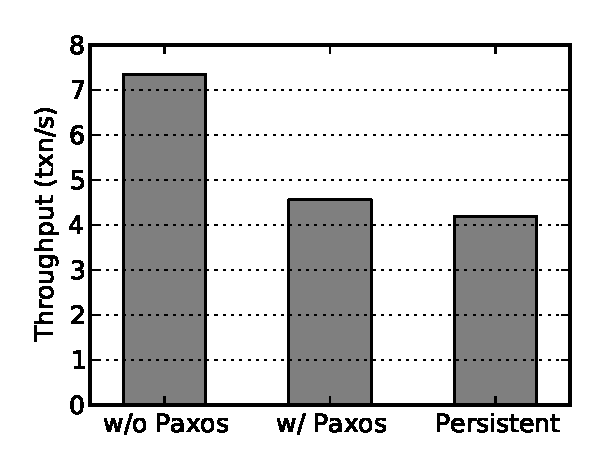
\includegraphics[width=0.6\columnwidth]{figs/paxos_persistent.pdf}
    \caption{
		Performance overhead of paxos protocol and persistent storage.
	}
	\label{fig:paxos-persistent}
\end{figure}

\cref{fig:paxos-persistent} also shows the overhead of writing the 
records to persistent storage, thus tolerate system crashes. It turns 
out that the disk writing overhead is smaller than the overhead of 
paxos protocol. 

\subsection{Locking Granularity}

\begin{figure}[t!]
	\centering
	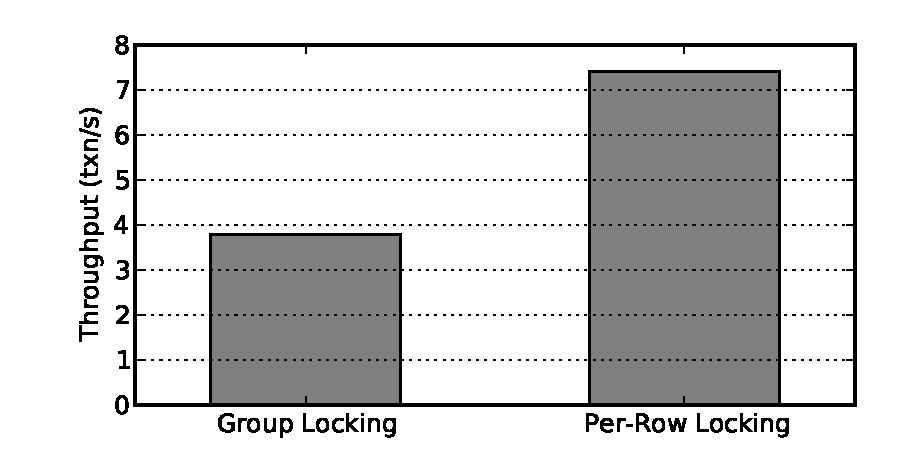
\includegraphics[width=0.6\columnwidth]{figs/locking_granularity.pdf}
    \caption{
		Performance comparison between different locking granularity.
	}
	\label{fig:locking-granularity}
\end{figure}

In \cref{fig:locking-granularity}

\section{Discussion}


% The following two commands are all you need in the
% initial runs of your .tex file to
% produce the bibliography for the citations in your paper.
\bibliographystyle{abbrv}
\bibliography{vldb_sample}  % vldb_sample.bib is the name of the Bibliography in this case
% You must have a proper ".bib" file
%  and remember to run:
% latex bibtex latex latex
% to resolve all references

\subsection{References}
Generated by bibtex from your ~.bib file.  Run latex,
then bibtex, then latex twice (to resolve references).




\end{document}
